\subsection{Zusammenfassung Skinning}

Skinning verfolgt das Ziel, dass sich ein Modell nat\"urlich bei jeder Bewegung des Skelettes sinnvoll mit bewegt. Das wird durch viele Faktoren beeinflusst, wie zum Beispiel durch das Material der Figur oder durch die physikalischen Gesetze des Films. Es gibt viele Ans\"atze - vom Einsatz komplexer Hardware, um physiologisch komplizierte Prozesse wie das Atmen darzustellen, bis hin zu einfachen geometrischen Ans\"atzen. 

Diese Ans\"atze basieren auf der Grundlage, die Transformationen nach physiologischen Eigenschaften zu modifizieren. Das prim\"are Beispiel hierf\"ur ist wohl die Vergabe von Gewichten an einzelne Punkte auf der Haut, um die Abh\"angigkeit von mehreren Knochen zu simulieren. 

Im Bereich des geometrischen Skinning ist Linear Blend Skinning auf Grund seiner Einfachheit und Performance der Standard. Dieser hat allerdings das Problem, durch Volumenverlust Artefakte zu erzeugen. Dual Quaternionen Blend Skinning behebt diese Problematik bei vergleichbarer Rechenleistung, erzeugt jedoch auch bei manchen Rotationen Artefakte und erlaubt keine Volumenver\"anderungen. Die beiden Verfahren nochmal im Vergleich bei unterschiedlicher Gewichtsverteilung in Abbildung 17.

\begin{figure}[thb]
	\centering
	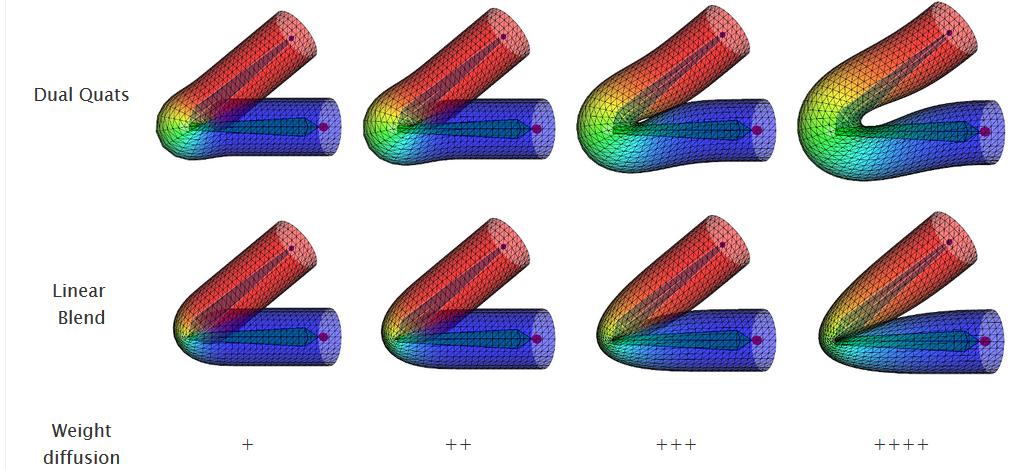
\includegraphics[width=\linewidth]{01_Skinning/pics/lbsvsdqs.png}
	\caption[Geometrisches Skinning im Vergleich]{Die erste Reihe zeigt Dual Quaternion Blend Skinning, die zweite Linear Blend Skinning. Die letzte Reihe bestellt die Gewichtsverteilung in jeder Spalte. Entnommen von \cite{weights}}
	\label{weights_fig1}
\end{figure}